\begin{enumerate}[label=\thesection.\arabic*.,ref=\thesection.\theenumi]
\numberwithin{equation}{enumi}

\item Sketch the Bode Magnitude and Phase plot for the following system. Also compute the gain margin and the phase margin.
\begin{align}
G\brak{s} &= \frac{10}{s\brak{1+0.5s}\brak{1+.01s}}
\label{eq:ee18btech11048_2}
\end{align}
\\
\solution 
The system is defined as follows:
\begin{align}
G\brak{s} &= \frac{10}{s\brak{1+0.5s}\brak{1+.01s}}
\end{align}
\begin{table}[!ht]
\centering
%%%%%%%%%%%%%%%%%%%%%%%%%%%%%%%%%%%%%%%%%%%%%%%%%%%%%%%%%%%%%%%%%%%%%%
%%                                                                  %%
%%  This is the header of a LaTeX2e file exported from Gnumeric.    %%
%%                                                                  %%
%%  This file can be compiled as it stands or included in another   %%
%%  LaTeX document. The table is based on the longtable package so  %%
%%  the longtable options (headers, footers...) can be set in the   %%
%%  preamble section below (see PRAMBLE).                           %%
%%                                                                  %%
%%  To include the file in another, the following two lines must be %%
%%  in the including file:                                          %%
%%        \def\inputGnumericTable{}                                 %%
%%  at the beginning of the file and:                               %%
%%        \input{name-of-this-file.tex}                             %%
%%  where the table is to be placed. Note also that the including   %%
%%  file must use the following packages for the table to be        %%
%%  rendered correctly:                                             %%
%%    \usepackage[latin1]{inputenc}                                 %%
%%    \usepackage{color}                                            %%
%%    \usepackage{array}                                            %%
%%    \usepackage{longtable}                                        %%
%%    \usepackage{calc}                                             %%
%%    \usepackage{multirow}                                         %%
%%    \usepackage{hhline}                                           %%
%%    \usepackage{ifthen}                                           %%
%%  optionally (for landscape tables embedded in another document): %%
%%    \usepackage{lscape}                                           %%
%%                                                                  %%
%%%%%%%%%%%%%%%%%%%%%%%%%%%%%%%%%%%%%%%%%%%%%%%%%%%%%%%%%%%%%%%%%%%%%%



%%  This section checks if we are begin input into another file or  %%
%%  the file will be compiled alone. First use a macro taken from   %%
%%  the TeXbook ex 7.7 (suggestion of Han-Wen Nienhuys).            %%
\def\ifundefined#1{\expandafter\ifx\csname#1\endcsname\relax}


%%  Check for the \def token for inputed files. If it is not        %%
%%  defined, the file will be processed as a standalone and the     %%
%%  preamble will be used.                                          %%
\ifundefined{inputGnumericTable}

%%  We must be able to close or not the document at the end.        %%
	\def\gnumericTableEnd{\end{document}}


%%%%%%%%%%%%%%%%%%%%%%%%%%%%%%%%%%%%%%%%%%%%%%%%%%%%%%%%%%%%%%%%%%%%%%
%%                                                                  %%
%%  This is the PREAMBLE. Change these values to get the right      %%
%%  paper size and other niceties.                                  %%
%%                                                                  %%
%%%%%%%%%%%%%%%%%%%%%%%%%%%%%%%%%%%%%%%%%%%%%%%%%%%%%%%%%%%%%%%%%%%%%%

	\documentclass[12pt%
			  %,landscape%
                    ]{report}
       \usepackage[latin1]{inputenc}
       \usepackage{fullpage}
       \usepackage{color}
       \usepackage{array}
       \usepackage{longtable}
       \usepackage{calc}
       \usepackage{multirow}
       \usepackage{hhline}
       \usepackage{ifthen}

	\begin{document}


%%  End of the preamble for the standalone. The next section is for %%
%%  documents which are included into other LaTeX2e files.          %%
\else

%%  We are not a stand alone document. For a regular table, we will %%
%%  have no preamble and only define the closing to mean nothing.   %%
    \def\gnumericTableEnd{}

%%  If we want landscape mode in an embedded document, comment out  %%
%%  the line above and uncomment the two below. The table will      %%
%%  begin on a new page and run in landscape mode.                  %%
%       \def\gnumericTableEnd{\end{landscape}}
%       \begin{landscape}


%%  End of the else clause for this file being \input.              %%
\fi

%%%%%%%%%%%%%%%%%%%%%%%%%%%%%%%%%%%%%%%%%%%%%%%%%%%%%%%%%%%%%%%%%%%%%%
%%                                                                  %%
%%  The rest is the gnumeric table, except for the closing          %%
%%  statement. Changes below will alter the table's appearance.     %%
%%                                                                  %%
%%%%%%%%%%%%%%%%%%%%%%%%%%%%%%%%%%%%%%%%%%%%%%%%%%%%%%%%%%%%%%%%%%%%%%

\providecommand{\gnumericmathit}[1]{#1} 
%%  Uncomment the next line if you would like your numbers to be in %%
%%  italics if they are italizised in the gnumeric table.           %%
%\renewcommand{\gnumericmathit}[1]{\mathit{#1}}
\providecommand{\gnumericPB}[1]%
{\let\gnumericTemp=\\#1\let\\=\gnumericTemp\hspace{0pt}}
 \ifundefined{gnumericTableWidthDefined}
        \newlength{\gnumericTableWidth}
        \newlength{\gnumericTableWidthComplete}
        \newlength{\gnumericMultiRowLength}
        \global\def\gnumericTableWidthDefined{}
 \fi
%% The following setting protects this code from babel shorthands.  %%
 \ifthenelse{\isundefined{\languageshorthands}}{}{\languageshorthands{english}}
%%  The default table format retains the relative column widths of  %%
%%  gnumeric. They can easily be changed to c, r or l. In that case %%
%%  you may want to comment out the next line and uncomment the one %%
%%  thereafter                                                      %%
\providecommand\gnumbox{\makebox[0pt]}
%%\providecommand\gnumbox[1][]{\makebox}

%% to adjust positions in multirow situations                       %%
\setlength{\bigstrutjot}{\jot}
\setlength{\extrarowheight}{\doublerulesep}

%%  The \setlongtables command keeps column widths the same across  %%
%%  pages. Simply comment out next line for varying column widths.  %%
\setlongtables

\setlength\gnumericTableWidth{%
	55pt+%
	35pt+%
	119pt+%
0pt}
\def\gumericNumCols{3}
\setlength\gnumericTableWidthComplete{\gnumericTableWidth+%
         \tabcolsep*\gumericNumCols*2+\arrayrulewidth*\gumericNumCols}
\ifthenelse{\lengthtest{\gnumericTableWidthComplete > \linewidth}}%
         {\def\gnumericScale{\ratio{\linewidth-%
                        \tabcolsep*\gumericNumCols*2-%
                        \arrayrulewidth*\gumericNumCols}%
{\gnumericTableWidth}}}%
{\def\gnumericScale{1}}

%%%%%%%%%%%%%%%%%%%%%%%%%%%%%%%%%%%%%%%%%%%%%%%%%%%%%%%%%%%%%%%%%%%%%%
%%                                                                  %%
%% The following are the widths of the various columns. We are      %%
%% defining them here because then they are easier to change.       %%
%% Depending on the cell formats we may use them more than once.    %%
%%                                                                  %%
%%%%%%%%%%%%%%%%%%%%%%%%%%%%%%%%%%%%%%%%%%%%%%%%%%%%%%%%%%%%%%%%%%%%%%

\ifthenelse{\isundefined{\gnumericColA}}{\newlength{\gnumericColA}}{}\settowidth{\gnumericColA}{\begin{tabular}{@{}p{55pt*\gnumericScale}@{}}x\end{tabular}}
\ifthenelse{\isundefined{\gnumericColB}}{\newlength{\gnumericColB}}{}\settowidth{\gnumericColB}{\begin{tabular}{@{}p{35pt*\gnumericScale}@{}}x\end{tabular}}
\ifthenelse{\isundefined{\gnumericColC}}{\newlength{\gnumericColC}}{}\settowidth{\gnumericColC}{\begin{tabular}{@{}p{119pt*\gnumericScale}@{}}x\end{tabular}}

\begin{tabular}[c]{%
	b{\gnumericColA}%
	b{\gnumericColB}%
	b{\gnumericColC}%
	}

%%%%%%%%%%%%%%%%%%%%%%%%%%%%%%%%%%%%%%%%%%%%%%%%%%%%%%%%%%%%%%%%%%%%%%
%%  The longtable options. (Caption, headers... see Goosens, p.124) %%
%	\caption{The Table Caption.}             \\	%
% \hline	% Across the top of the table.
%%  The rest of these options are table rows which are placed on    %%
%%  the first, last or every page. Use \multicolumn if you want.    %%

%%  Header for the first page.                                      %%
%	\multicolumn{3}{c}{The First Header} \\ \hline 
%	\multicolumn{1}{c}{colTag}	%Column 1
%	&\multicolumn{1}{c}{colTag}	%Column 2
%	&\multicolumn{1}{c}{colTag}	\\ \hline %Last column
%	\endfirsthead

%%  The running header definition.                                  %%
%	\hline
%	\multicolumn{3}{l}{\ldots\small\slshape continued} \\ \hline
%	\multicolumn{1}{c}{colTag}	%Column 1
%	&\multicolumn{1}{c}{colTag}	%Column 2
%	&\multicolumn{1}{c}{colTag}	\\ \hline %Last column
%	\endhead

%%  The running footer definition.                                  %%
%	\hline
%	\multicolumn{3}{r}{\small\slshape continued\ldots} \\
%	\endfoot

%%  The ending footer definition.                                   %%
%	\multicolumn{3}{c}{That's all folks} \\ \hline 
%	\endlastfoot
%%%%%%%%%%%%%%%%%%%%%%%%%%%%%%%%%%%%%%%%%%%%%%%%%%%%%%%%%%%%%%%%%%%%%%

\hhline{|-|-}
	 \multicolumn{1}{|p{\gnumericColA}|}%
	{\gnumericPB{\centering}\textbf{Zeros}}
	&\multicolumn{1}{p{\gnumericColB}|}%
	{\gnumericPB{\centering}\textbf{Poles}}

\\
\hhline{|---|}
	 \multicolumn{1}{|p{\gnumericColA}|}%
	{\gnumericPB{\centering}-}
	&\multicolumn{1}{p{\gnumericColB}|}%
	{\gnumericPB{\centering}0}

\\
\hhline{|---|}
	 \multicolumn{1}{|p{\gnumericColA}|}%
	{\gnumericPB{\centering} }
	&\multicolumn{1}{p{\gnumericColB}|}%
	{\gnumericPB{\centering}-2}

\\
\hhline{|---|}
	 \multicolumn{1}{|p{\gnumericColA}|}%
	{\gnumericPB{\centering} }
	&\multicolumn{1}{p{\gnumericColB}|}%
	{\gnumericPB{\centering}-100}

\\
\hhline{|-|-|-|}
\end{tabular}

\ifthenelse{\isundefined{\languageshorthands}}{}{\languageshorthands{\languagename}}
\gnumericTableEnd

\caption{Zeros and Poles}
\label{table:ee18btech11048}
\end{table}\\
The magnitude and phase plot are as follows: Fig\ref{fig:ee18btech11048} 
\begin{figure}[!h]
\centering
  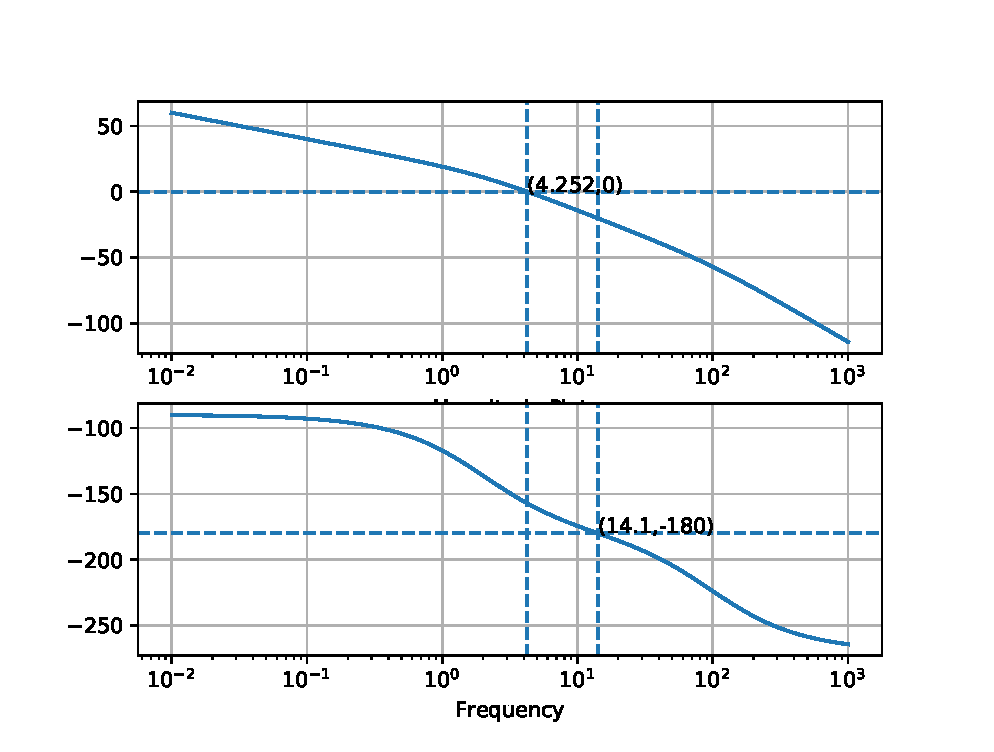
\includegraphics[width=\columnwidth]{./figs/ee18btech11048.eps}
  \caption{Graphs}
  \label{fig:ee18btech11048}
\end{figure}

The python code to obtain the graphs:

\begin{lstlisting}
codes/ee18btech11048.py
\end{lstlisting}

\item Finding the Phase Margin \brak{PM}.
\begin{align}
G\brak{j\omega} &= \frac{10}{j\omega\brak{1+0.5j\omega}\brak{1+.01j\omega}}
\end{align}
\begin{align}
{\em PM} = \angle G(\j\omega_{gc}) + 180\degree 
\end{align}\\
 where $\omega_{gc}$ is frequency when gain = 1 .\\
\solution
\begin{align}
    \frac{100}{\omega\sqrt{\brak{0.5\omega}^2+1}\sqrt{\brak{0.01\omega}^2+1}} &= 1
\label{eq:ee18btech11048_2}
\end{align}{}
Solving Eq. \eqref{eq:ee18btech11048_2} {\em or} from Fig \ref{fig:ee18btech11048} :

\begin{align}
\implies
\omega_{gc} &= 4.25  \\
\angle G\brak{\j\omega_{gc}} &= -157.2 \\
\implies
PM &= 22.8 
\end{align}

\item Finding the Gain Margin \brak{GM}\\
\begin{align}
{\em GM} = 0\degree -G(\j\omega_{pc}) db 
\end{align}
 where $\omega_{pc}$ is frequency when phase = -180\degree
\\
\solution

\begin{multline}
\arctan \brak{0}-\arctan \brak{\frac{\omega}{0}} - \arctan \brak{\frac{\omega}{2}}- \\\arctan \brak{\frac{\omega}{100}} = -180\degree
\label{eq:ee18btech11048_3}
\end{multline}
Solving Eq. \eqref{eq:ee18btech11048_3} {\em or} from Fig \ref{fig:ee18btech11048} :

\begin{align}
\implies
\omega &=  14.1  \\
-G(\j\omega) db = -20.2 \\
\implies
GM &= 20.2 db
\end{align}

\end{enumerate}
